Now having three successfull models that are able to prediction GFP fluorescence from the whole cell, nuclei and ER, one can combine their predictions together for the same image. For that an output RGB image was contructed, where each prediction takes one channel. In this case channel correspondence is the following: red --- ER, green --- GFP, blue --- nuclei. The resulting image is shown in Figure \ref{fig:combined}. Additionally one can see, that GFP model has successfully generalized on other cell phenotypes (CHOZN, PHX), although it was train on H19 only.
\begin{figure}[htb]
	\begin{center}
		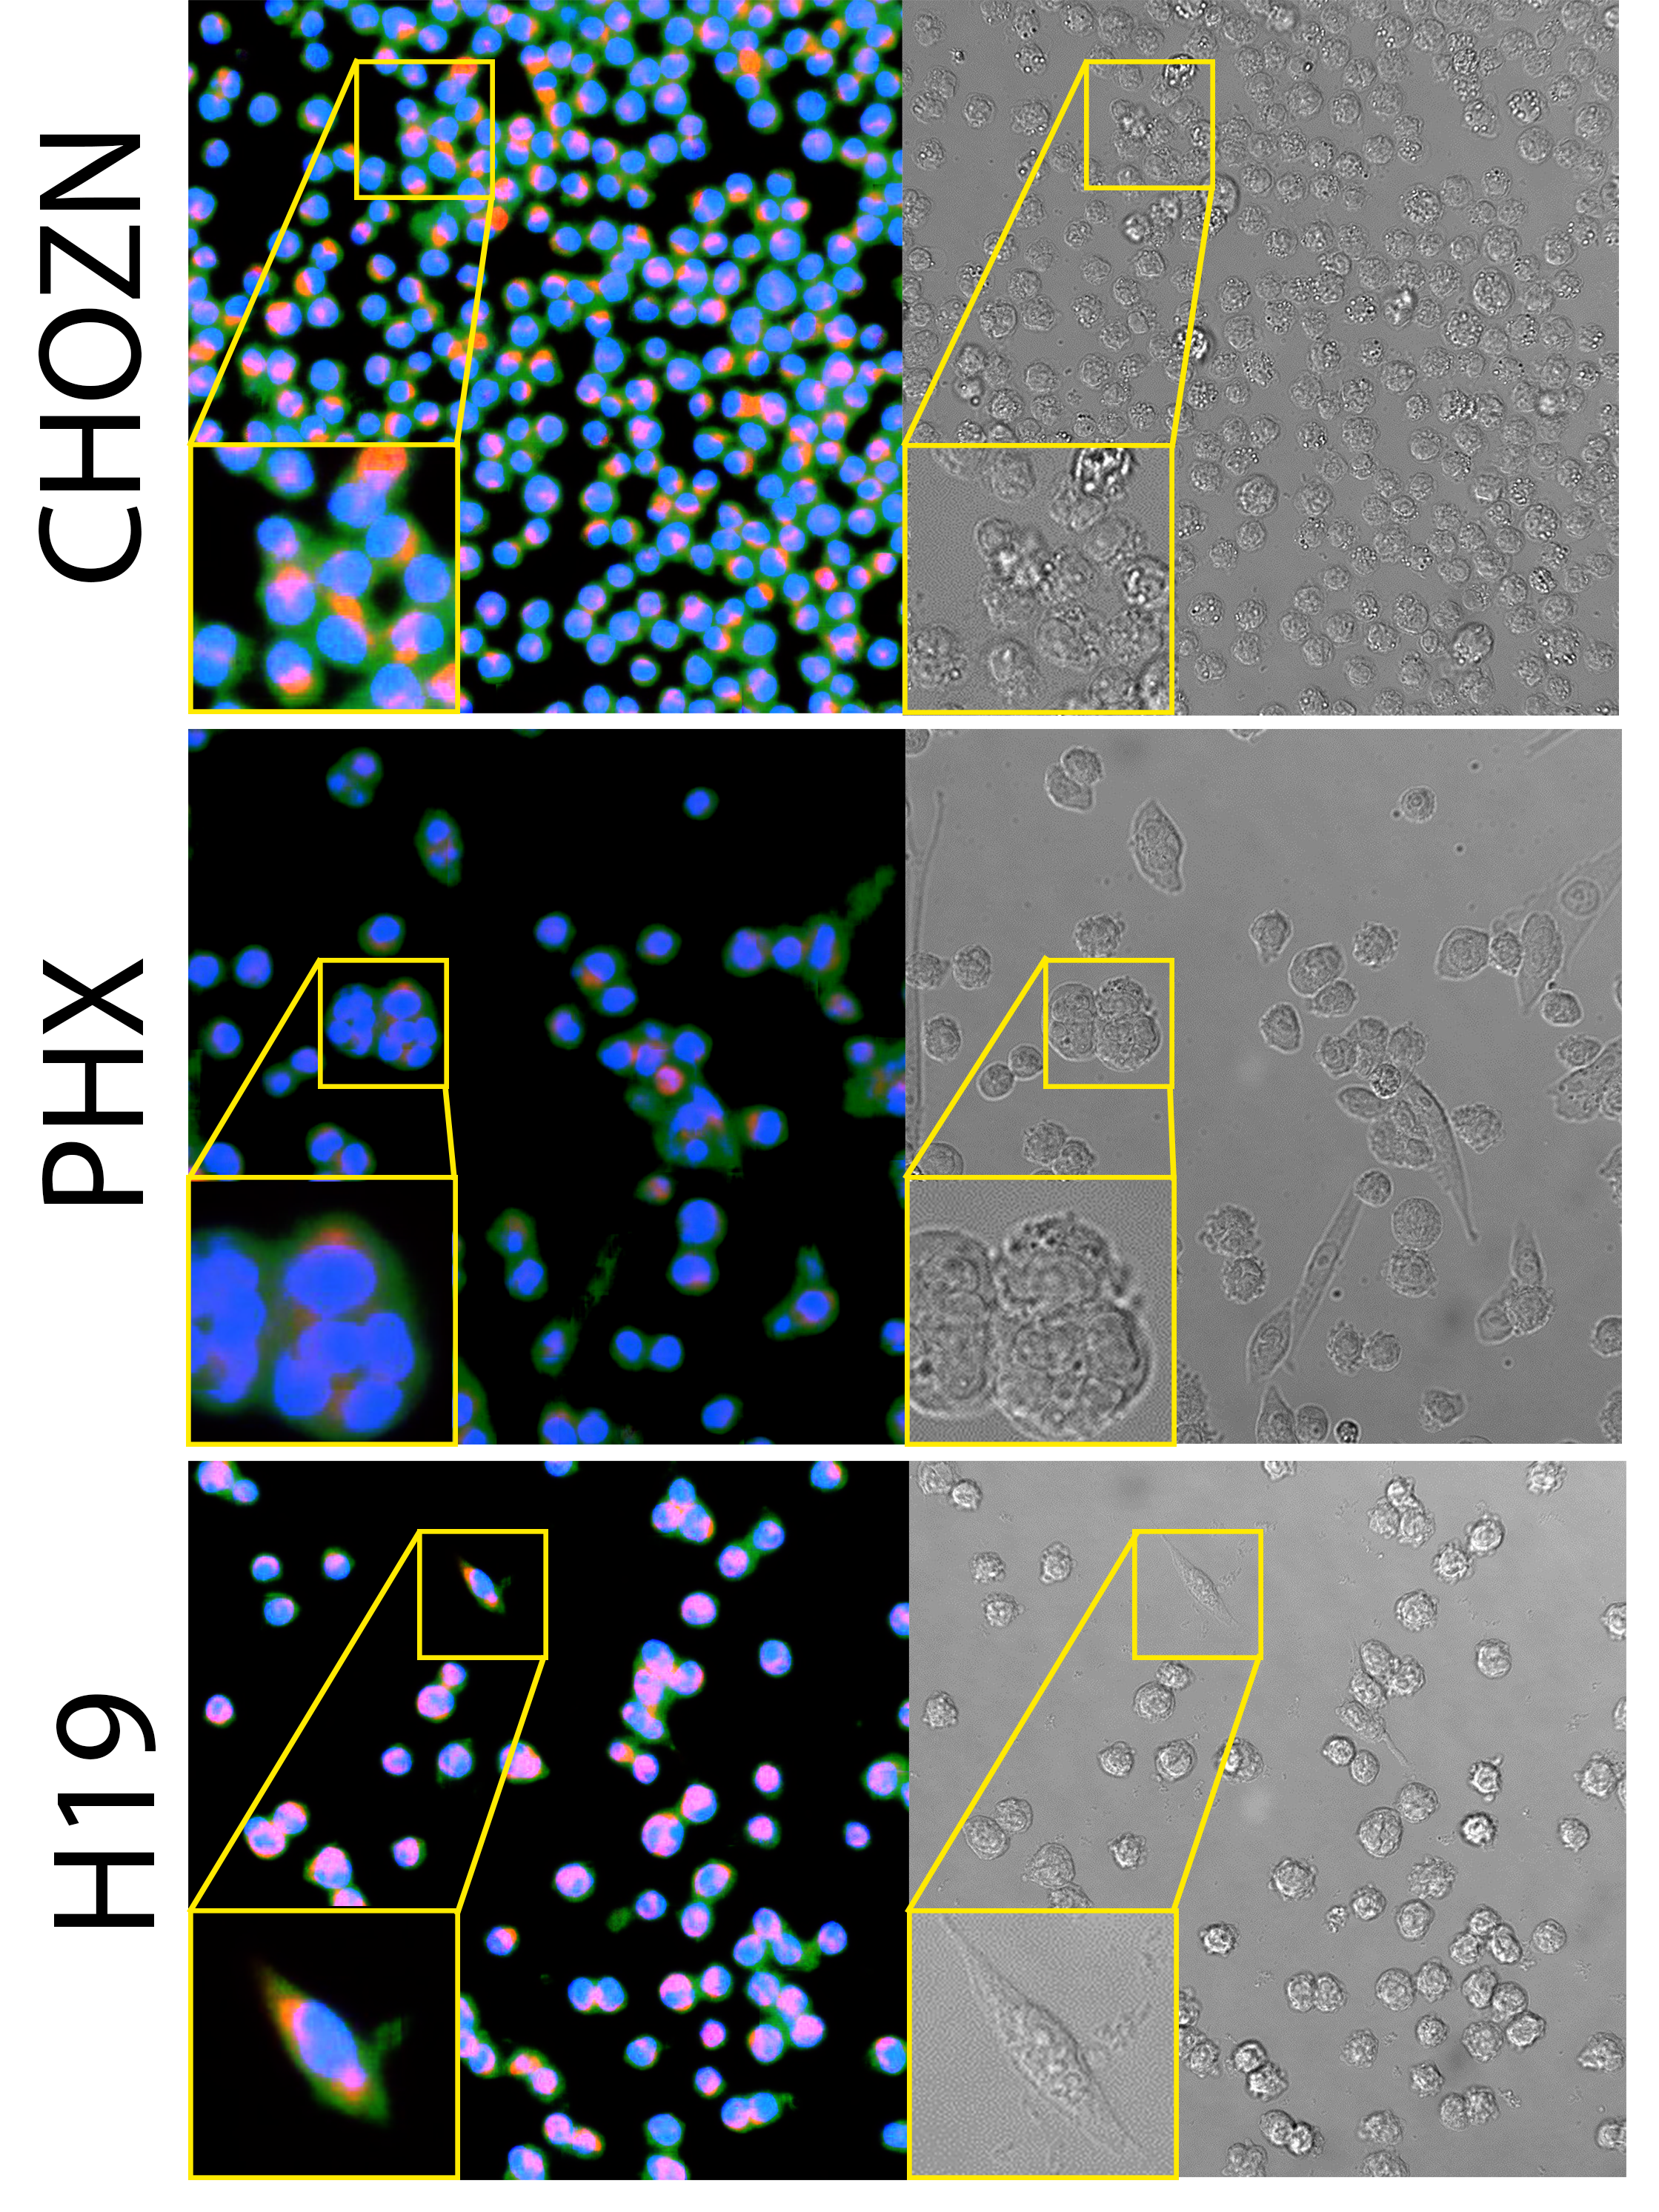
\includegraphics[width=0.4\linewidth]{bilder/combined/combined.png}
		\caption{GFP, Nuclei and ER combined}\label{fig:combined}
	\end{center}
\end{figure}
